\documentclass{article}
\usepackage{tikz}
\usetikzlibrary{matrix}
\begin{document}
\section{A picture}
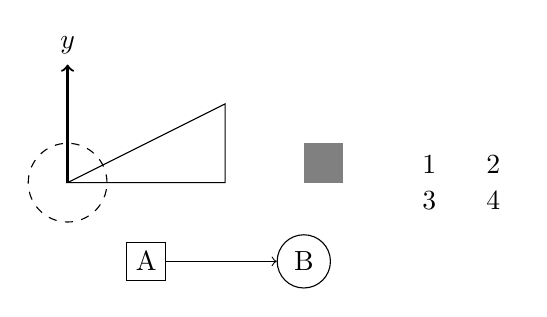
\begin{tikzpicture}
\draw (0,0) -- (2,0) -- (2,1) -- cycle;
\draw[thick,->] (0,0) -- (0,1.5) node[above] {$y$};
\draw[dashed] (0,0) circle (0.5cm);
\fill[gray] (3,0) rectangle (3.5,0.5);
\node[draw] (a) at (1,-1) {A};
\node[draw,circle] (b) at (3,-1) {B};
\draw[->] (a) -- (b);
\matrix[matrix of nodes,column sep=4mm] at (5,0) {
  1 & 2 \\
  3 & 4 \\
};
\end{tikzpicture}
\end{document}
